\documentclass[12pt]{article} 
\usepackage{geometry} %页边距设置等

%-----------------------------format.tex-----------------
\usepackage{amsmath,amssymb} 
\usepackage{graphicx}
\usepackage{fancybox}
\usepackage{fancyhdr} 
\usepackage{lastpage}
\usepackage{hyperref}
\hypersetup{
    unicode={true},pdfstartview={FitH},pdfborder={0 0 0},
    colorlinks,linkcolor=black,citecolor=black,hyperindex,plainpages=false,}   %目录超链接格式设置
% style: page layout
\setlength{\headheight}{15pt}
\setlength{\headsep}{20pt}
\setlength{\footskip}{30pt}
\setlength{\voffset}{-5pt}
\setlength{\hoffset}{16pt}
\setlength{\oddsidemargin}{0pt}
\setlength{\evensidemargin}{\oddsidemargin}
\setlength{\marginparpush}{0pt}
\setlength{\marginparwidth}{0pt}
\addtolength{\textheight}{3\baselineskip}

% Definitions的格式设置
\newtheorem{definition}{{definition}}
\newcounter{numdefinition}
\renewenvironment{definition}[1]
{\noindent\stepcounter{numdefinition}
\slshape Definition \arabic{numdefinition} \textsf{#1 :}
\begin{quote}\small\itshape}
{\end{quote}}

\newcommand{\dd}{\ensuremath{\,\mathrm{d}}}
%===============================================================
\fancypagestyle{plain}%重新定义plain格式,用于summary sheet
{\fancyhf{}
\setlength{\headheight}{0pt}\setlength{\headsep}{0pt}
\setlength{\voffset}{-50pt}\setlength{\oddsidemargin}{0pt}}

\graphicspath{{pic/}}
%=========================定义页眉===============================
\pagestyle{fancy} 
\lhead{page\thepage\ of \pageref{LastPage}}
\chead{} \rhead{Team \footnotesize{\#} 6406} \lfoot{}
\cfoot{\thepage}
\rfoot{}
\renewcommand{\headrulewidth}{0pt}

\begin{document}

%=========================summary sheet.tex========================

\thispagestyle{empty}
\begin{minipage}{0.3\textwidth}
\begin{flushleft}
For office use only\\
   T1\ \rule{3cm}{0.5pt}\\
   T2\ \rule{3cm}{0.5pt}\\
   T3\ \rule{3cm}{0.5pt}\\
   T4\ \rule{3cm}{0.5pt}\\
\end{flushleft}
\end{minipage}\hspace{\fill}
\begin{minipage}{0.3\textwidth}
\centering
Team Control Number\\[5pt]
\fontsize{36pt}{\baselineskip}\selectfont  \textbf{666} \normalsize\\[10pt]
Problem Chosen\\[5pt]
\fontsize{18pt}{\baselineskip}\selectfont \textbf{A }\normalsize\\
\end{minipage}\hfill
\begin{minipage}{0.35\textwidth}
\begin{flushright}
\shortstack[l]{
For office use only\\
   F1\ \rule{3cm}{0.5pt}\\
   F2\ \rule{3cm}{0.5pt}\\
   F3\ \rule{3cm}{0.5pt}\\
   F4\ \rule{3cm}{0.5pt}}
\end{flushright}
\end{minipage}\vspace*{10pt}
\rule{\textwidth}{0.5pt}

\begin{center}
  \textbf{2010 Mathematical Contest in Modeling (MCM) Summary Sheet}
\end{center}
%\enlargethispage
\noindent
{\Large \textbf{Summary}}
\vspace{7pt}

%==========================abstract.tex================================
Firstly, the ``sweet spot'' on a bat is defined as
the very spot where the maximum power is transferred to the ball in the collision process.

In order to locate the sweet spot of a bat, we
model the bat approximately as a rigid, free object and
the ball as a linear spring with friction in collision process
which is considered as an one-dimensional problem. This
is our basic model, in which the exit velocity of the ball is
a function of some factors, including masses of ball and
bat, centers of those masses, moment of inertia of the bat, initial
velocity of the ball and the bat, coefficient of restitution
and the location of impact point.
With specific values of these factors given, the exit speed
of ball is only an explicit function depended on the
location of impact point. A graph drawn by MATLAB$^\circledR$ shows the relationship between exit velocity of the ball and location of the impact point.Since the peak point of the curve in the graph is not corresponding to the end of the bat, we draw a conclusion that sweet spot is not located at the end of the bat.After this,an additionally physical explanation is put forward.

In order to predict the effect of ``corking'' more accurate, the vibration of bat is taken into account and then a generalized model is proposed. Here \emph{finite element method} is used to study the vibration of the whole bat, and an effective coefficient of COR is given to describe the energy dissipation of the vibration of bat. Then we obtain an improved formula to describe the relationship of factors above. According to the new formula, a comparison graph on the normal bat and the corked bat is plotted. By this graph, we can conclude that corking does not enhance ``sweet spot'' effect, while it is prolonged the reaction time and easier for batter to control bat. This answers why corking is forbidden. A more detailed physical explanation is presented in this report.

The augmented model is used to predict the behavior of wood and metal bat. With experimental data of parameters for ash and aluminum bats, we draw a figure of exit velocity of ball corresponding to the location of the impact point. By this figure and the discussion of energy's transfer process, we find that there are some significant different behaviors between the wood bat and the metal bat. It shows that the metal bat outperforms the wood one remarkably. This is the main reason for the prohibition of metal bats.

%\textbf{keyword}: sweet spot; corked bat; coefficient of restitution;%xxx speed; finite element method; 
\newpage

%====================目录页========================================
\thispagestyle{empty}
\setcounter{page}{0}
{\begin{center}\Large \textbf{Dynamic Model of ``Sweet Spot Effect''}\end{center}}
\tableofcontents                                                  %
\newpage                                                          %
%==================================================================

\newcommand{\vw}{\frac{v_i}{\omega_i}}

%=======================\input{introduction1}=======================
\section{Introduction}

The game of baseball has a certain fascination for physicists.
There have been numerous papers in the literature addressing a wide
variety of issues amenable to a physics calculation.

In all the studies,the hottest areas include the standardization of the game and its equipments;the aerodynamics of a spinning baseball; the peculiar behavior of the knuckleball; the coefficient of restitution of a baseball and its effect on the bounce of the ball off the bat; and the dynamics of the ball-bat collision and sweet spot. It is this latter topic that is the subject of this paper.

Given the popularity of baseball and the natural curiosity
of physicists to understand collision phenomena, it is surprising
that very few measurements have ever been made on the
behavior of a baseball bat when it impacts with a ball.

Most of the studies on ball-bat collision is experimental, mainly because precisely theoretical study of the collision process is very difficult.The collision can be very violent,and the impact time is very short,resulting in the complexity of the problem.

There are some theoretical on ball-bat collision,most of which are based on values of parameters obtained from previous experimental study.It is impossible to do study totally independent of experiments on such a
practical problem,although only principles of classical mechanics is involved.

Alan M.Nathan,Van Zandt and H.Brody have done a lot of studies on baseball,and on the collision medel.R.K.Adair published a popular book discussing the physics of baseball in all.Our study here is mainly conducted on the basis of their research, also contains many others' work.

%============================\input{definitions1}===========
\section{Definitions}
\begin{definition}{Sweet Spot}
 The "sweet spot" on a bat is defined as the very spot where the maximum power of the collision system is transferred to the ball in the collision process.
\end{definition}

\begin{definition}{Center of Percussion (COP)}
A point conjugate to the point on the handle where the bat is held.
A ball that strikes the stationary bat between the COP and
the handle tends to drive the handle in the direction of the ball's motion.
A ball that strikes the the end of the bat beyond the COP tends to drive
the handle forward, opposite to the direction of the ball.
A ball that strikes the COP has no effect on the handle.
\end{definition}

\begin{definition}{Coefficient of Restitution (COR)}
The ratio of the velocity of the ball rebounding from the surface of a hard,
immovable object to its incident velocity.
Consequently, the COR is equal to the square root of the proportion of the collision
energy returned to  the kinetic energy of the ball's flight.
We use COR of the bat-ball collision so as to take into account
the loss of mechanical energy in the inelastic collision
\end{definition}

%=======================\input{Assumptions1}=====================================
\section{Assumptions}
\begin{enumerate}
\item The bat is rigid, so there is no vibration in the bat(for the basic model).
\item The ball hit and rebound perpendicular to the bat and is in the plane of the swing.
\item The ball can be considered as a linear spring with friction.
\item The bat is a free object in collision,and both ends of the bat is completely free.
\item The vibration of the bat is harmonic(for augmented model).
\end{enumerate}

%=====================\input{symbols}==========================================
\section{Symbols}

\begin{tabular}{ll}
\hline
symbols&definitions\\
\hline
$v_i$& velocity of ball before collision\\
$v_f$& velocity of ball after collision\\
$V_f$& velocity of bat after collision\\
$S$ & the shear modulus the bat\\
$Y$ & Young’s modulus of the bat\\
$\rho$ & the density of the bat\\
$A_i$ & cross-sectional area of each slices of the bat\\
$\Delta z$ & the thickness of each segment of the bat\\
$y_i(z)$ & the transverse displacement of each segment of the bat\\
$\phi$ & orientation of each segment of the bat\\
$\Phi$ & $\Phi_i=\phi_i\Delta z$\\
$I_i$ & area moment of inertia of slice $i$  (about an axis\\
      &passing through the center of mass of the slice and
       normal to the $y-z$ plane)\\
$b$& the distance between the inpact point and CM\\
$m$ & mass of the ball\\
$M$ & mass of the bat\\
$e_0$ & Coefficient of restitution (COR),defined as
	$e_0\equiv {v_{rel,f}}/{v_{rel,b}}$\\
\hline
\end{tabular}

%=============================\input{ModelforCollision}==========================
\section{Model for Bat-ball Collision}

When a ball strikes a baseball bat held firmly by the
hands, the bat transfers vibrational energy to the hands, and
the hands exert an impulsive reaction force on the handle.
This force is usually neglected when modeling the dynamics
of the collision, since it is usually assumed that the ball will
leave the bat before the impulse is transmitted to the
hands \cite{CrossSeptember1998}\cite{H.Brody1986}\cite{Zandt1992}.
It is probably better to treat the bat as a free-body,
rather than an object clamped at one end.

The force between the ball and bat in the collision process
can be very large, while the gravity is so small that it is negligible.
For a long home run, the force on the ball reaches a value of near 9000 pounds\cite{K.Adair2002}.

The collision is simplified as a moving free object collides with a spring with friction.

%friction or 弹性? 产生的热能主要是弹性导致,还是bat-ball之间的摩擦?
%我认为,主要是弹性导致的,ball内部分子之间的摩擦导致产热
%所以,从宏观上看,碰撞的问题不涉及摩擦问题。

\subsection{Calculation for the maximum power point}

For this part of the calculation,
we follow nearly exactly the work of H.Brody\cite{H.Brody1986},
who calculate the maximum power point of ball-bat collision.

it is assumed that the ball hit and rebound perpendicular to the bat and is in the plane of the swing.

\begin{center}
\begin{figure}[htpb]
\centering
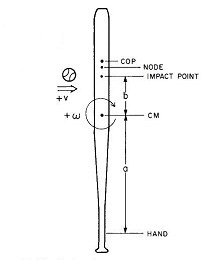
\includegraphics[scale=0.8]{locationofpoint}
\caption{location of point}\label{fig:locationofpoint}
\end{figure}
\end{center}

The three equations below come from
conservation of linear momentum,
conservation of angular momentum,
and the definition of coefficient restitution.
The angular velocity $\omega$ is taken about the bat CM
and clockwise is defined as positive,
as shown in Fig.\ref{fig:locationofpoint}
This is all in the frame of reference
moving with the initial velocity of the CM of the bat
and the bat is considered a free-body.

\begin{eqnarray}
m\cdot v_i=m\cdot v_f+M\cdot V_f \\
b\cdot m\cdot v_i+I\cdot \omega_i=b\cdot m\cdot v_f+I\cdot \omega_f\\
e_0\cdot (v_i-\omega_i\cdot b)=V_f+\omega_f\cdot b-v_f
\end{eqnarray}
Where $m$ and $M$ are the ball and bat mass,
$v$ and $V$ are the ball and bat velocity(initial and final),
$\omega$ is the bat angular velocity(initial and final),
and $e$ is the coefficient of restitution.

Here, we use COR of the bat-ball collision so as to take into account
the loss of mechanical energy in the inelastic collision{非弹性碰撞}.

Solving these three equations for $v_f$ by eliminating $V_f$ and $w_f$ gives

\begin{equation}
v_f=v_i-\frac{(1+e_0)\cdot(v_i-\omega_i\cdot b)}{1+m/M+(m\cdot b^2/I)}
\end{equation}

Note that when $w_i=0$, this expression is a function of $b^2$,
so it must have an extremum (maximum in this case) at $b=0$,
the center of mass of the bat.
%为何冒出这一句话?
This is, of course, expected, since if the bat has no initial rotational energy, a
hit at the CM will give it no final rotational energy.

To find the value of $b$ which maximizes $v_f$ in the general case, the
expression for $v_f$ is differentiated with respect to $b$
and set the result equal to zero.

\begin{equation}
\omega_i\cdot b^2-2v_i\cdot b-[\omega_i\cdot (M+m)\cdot I]/(m\cdot M)
\end{equation}

Solve this equation, we can get b:

\begin{equation}
b=\vw\pm \sqrt{(\vw)^2+I\frac{m+M}{m\cdot M}}
\end{equation}

Since $v_i/\omega_i$ is negative,
the $+$ sign is to be used here on the square root.
The values of $m$, $M$, and $I$ are easy to obtain in the lab, while
the value of $w_i$ and $v_i$
are determined by the hitter swinging the
and the pitcher throwing the ball.

By then, the calculation of the location of
the maximum power spot by the model is finished. we
can get that the location $b$ is a function of ball/bat velocity ratio,
the masses of ball and bat, and
the moment of inertia of the bat with respect to CM.
the value of $b$ varies by these parameters.
The final velocity of the ball in the collision $v_f$
varies by the impact point location $b$
is drawn a graph with values obtained from experiments.
%Figure 3:final velocity $v_f$ varies by impact point location $b$

So it is obvious that maximum power spot is not at the end of the bat.




\subsection{Conclusion}
On the foundation of the collision model, we can draw a conclusion that the location of sweet point
is a function of ball/bat velocity ratio, the masses of ball and bat, and the moment of inertia of the bat
with respect to CM, and it varies by these parameters. As shown in fig.\ref{fig:maximum}, sweet spot
do not locate on the end of a bat, but locate on a point that has a certain distance to the end.

It is quite instructive to see how $b$ varies with each of these variables.
Consider if

$$I\cdot (m+M)\cdot \omega_i^2/(M\cdot m)\cdot v_i^2<1$$

the square root can be expanded and the result is

$$b=[(r+1)\cdot \omega_i\cdot k^2]/v_i$$

where $r=M/m$ and I has been replaced by $M\cdot k^2$.

This means that $b$, the distance from the CM of the bat to the impact point of the ball, increases as the
mass of the bat increases, increases as the moment of inertia of bat increases, and increases the more "wristy"
is the swing.

\begin{center}
\begin{figure}[htpb]
\centering
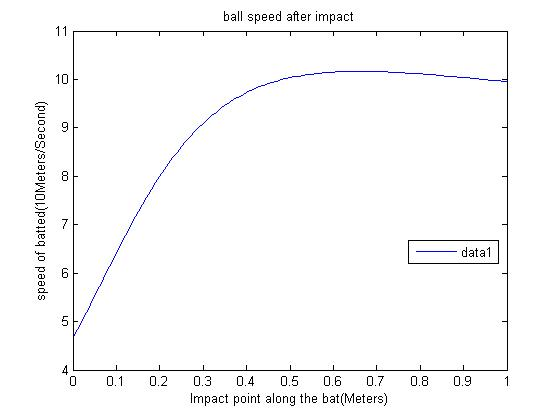
\includegraphics[scale=0.6]{firstwen}
\caption{final velocity $v_f$ varies by impact point location $b$}\label{fig:maximum}
\end{figure}
\end{center}

\subsection{The Physical Explanation}

Even though the velocity at the end of the bat is the largest, but
the speed of batted ball is also determined by the quantity
of mass near the impact point. In the end of the bat, the quantity
of mass nearby is almost half less since one side of the point is of no mass at
all. To gain a balance of the bat velocity and quantity of mass
nearby, it's acceptable that sweet spot locate not at the end, but a certain distance to the end.

%It is seemed to find the point at the end of the bat,
%for the lineal velocity of the impact point is maximum.
%it is obvious wrong according to our model,
%for there would be more energy loss in the form of thermal.

\subsection{Advice to the Batter}
\begin{enumerate}
\item You should hit a fast pitch closer to your hands for maximum power and you should try to hit a slow pitch
further out on your bat to get best results.
\item With a larger bat/ball mass ratio (hardball) hit the ball out further from the CM, and with a smaller bat/ball
mass ratio (softball) hit it closer to your hands.
\end{enumerate}

%===================\input{AugmentedModelofCollision}=============================================
\section{Augmented Model of Collision}

In the model above, we assumed that the bat is rigid and the vibration of the bat was neglected.
While actually, for the force in collision is very large(can reach 9000 pounds for a home run\cite{K.Adair2002}),
both the ball and the bat will be
distorted, and there must be vibration in the bat. In order to establish a more precise model in this part, the assumption of ``rigid bat'' is abandoned, and the vibration of the bat is taken into account. So the model of bat will be modified following. Then the model for collision is sure to be modified, while the model for the ball almost remains the same except that some of the expressions is displaced.

For this part of the calculation, we follow the model of Alan Nathan\cite{NathanNovember2000}, with some improvement in
the model of the ball according to the measurement of Kirkpatrick\cite{Kirkpatrick1963}.

\subsection{Model of Bat with Vibration}

\begin{center}
\begin{figure}[htpb]
\centering
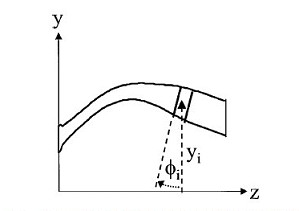
\includegraphics[scale=0.8]{batmodel}
\caption{Schematic{图解}
representation of a bat that is bent
and sheared.}\label{fig:batmodel}
\end{figure}
\end{center}

We start with Fig.\ref{fig:batmodel},
where we show schematically a baseball bat
that has been distorted from its equilibrium shape due to bending and shearing .
%我们用有限元的方法处理杆的运动学方程

We divide the bat into $N$ parallel slices of circular cross section,
each of thickness $\Delta z$ and each elastically coupled to its neighbors
through the Young's modulus $Y$ and the shear modulus $S$.
The distortion of each particular segment of the bat
can be characterized by its transverse displacement $y(z)$ and orientation $\phi(z)$
as a function of its coordinate $z$ along the long axis of the bat.

Based on the work of Van Zandt\cite{Zandt1992} and Alan Nathan\cite{NathanNovember2000},
we arrive at:

%公式1
\begin{eqnarray}
\ddot{y}_i&=&\frac{S}{\rho\Delta z^2}
[(y_{i+}+y_{i-1}-2y_i)+\frac{A_i-A_{i-1}}{A_i}  \label{equ:yddot}\\
&&(y_i-y_{i-1}+\Phi_{i-1})+(\Phi_i-\Phi_{i-1})] \nonumber\\
\ddot{\Phi}_i&=&\frac{Y}{\rho\Delta z^2}[(\Phi_{i+1}+\Phi_{i-1}-2\Phi_i)+
\frac{I_i-I_{i-1}}{I_i}(\Phi_i-\Phi_{i-1})] \nonumber \\
&&-\frac{S}{\rho I_i}[A_i(y_{i+1}-y{i-1}+\Phi_{i}+\Phi_{i-1}) \label{equ:phiddot} \\
&&-(A_{i}+A_{i-1})(y_{i}+y_{i-1}+\Phi_{i-1})]  \nonumber
\end{eqnarray}

where $\rho$, $A_i$, and $I_i$ are the density, cross-sectional area, and area moment of inertia of slice $i$
(about an axis passing through the center of mass of the slice and normal to the $y-z$ plane),
respectively, and $\Phi_i=\phi_i\Delta z$.

%All the bats we consider herein have a circular cross section.
For solid bats (such as a typical wood bat), a slice of radius $R_i$ has

\begin{eqnarray}
\left\{
\begin{array}{l}
A_i=\pi R_i^2\\
I_i=\pi{}R_i^4/4
\end{array}\right.
\end{eqnarray}

We assume that $\rho$, $Y$, and $S$ are uniform(independent of $i$).

We complete the statement of the problem by specifying the boundary conditions.
It is assumed that both ends of the bat are completely free\cite{H.Brody1990},
meaning that the force and torque on the end slices are due only to the next inner slices.
%We will show that this is a very good assumption for many purposes,
%including the calculation of the rebound velocity of the baseball.

In order to find the normal modes of the bat implied by our equations of motion,
we assume harmonic vibrations, so that

\begin{eqnarray}
\left\{
\begin{array}{l}
\ddot{y}_i=-\omega^2 y_i\\
\ddot{\Phi}_i=-\omega^2\Phi_i
\end{array}\right.
\end{eqnarray}

Then Eqs.\ref{equ:yddot}and \ref{equ:phiddot} can
be rewritten in a compact matrix notation as

$$H\psi =-\omega_n^2$$

where
\begin{center}
\begin{tabular}{rcl}
$\psi$&$\equiv$&
$\left(
  \begin{array}{c}
    y_{n1} \\
    \vdots\\
    y_{nN} \\
    \Phi_{n1}\\
    \vdots\\
    \Phi_{nN}\\
  \end{array}
\right)$
\end{tabular}
\end{center}
is a $2N$-element column matrix and $H$ is a nonsymmetric $2N\times 2N$ matrix.
One immediately recognizes this as an eigenvalue problem,
requiring the diagonalization of $H$ in order to find the normal mode
frequencies $\omega_n$ and associated eigenvectors $\psi_n$.

The lowest two modes are
zero-frequency rigid body modes corresponding to
uniform translation ($y_{ni}$ independent of $i$, $\phi_{ni}=0$) and
uniform rotation ($y_{ni}$ linear in $i$, $\phi_{ni}$ independent of $i$).

In the presence of a time-dependent external force on the $i$th slice,
an additional term $F_i(t)/(\rho A_i\Delta_z)$ appears on the right-hand-side of Eq.\ref{equ:yddot}.
Since the normal modes of the free vibration form a complete set, we write the solution as an expansion

$$y_i(t)=\sum_n a_n(t)y_{ni}$$

so that

\begin{equation}
\sum_n(\ddot{a}_n(t)+\omega^2_n a_n(t))y_{ni}=\frac{F_i(t)}{\rho A_i\Delta z}
\end{equation}

Using the orthogonality of the eigenstates,

$$\sum_I A_i y_{mi} y_{ni} \Delta z=\bar{A} \delta_{mn}$$

which defines $\bar{A}$,
we project out the $m$th mode to arrive at

%公式5
\begin{equation}
\ddot{a}_m(t)+\omega^2_m a_m(t)=\frac{1}{\rho \bar{A}}\sum_iF_i(t)y_{mi}
\end{equation}
%此时,a 的物理含义是什么?从展开式看。

In the ball-bat collision, the driving force $F_i(t)$ is the force
that the ball and bat mutually exert on each other. We next
turn to a discussion of the ball and a model for the force.


\subsection{Model of the Ball}

\begin{center}
\begin{figure}[htpb]
\centering
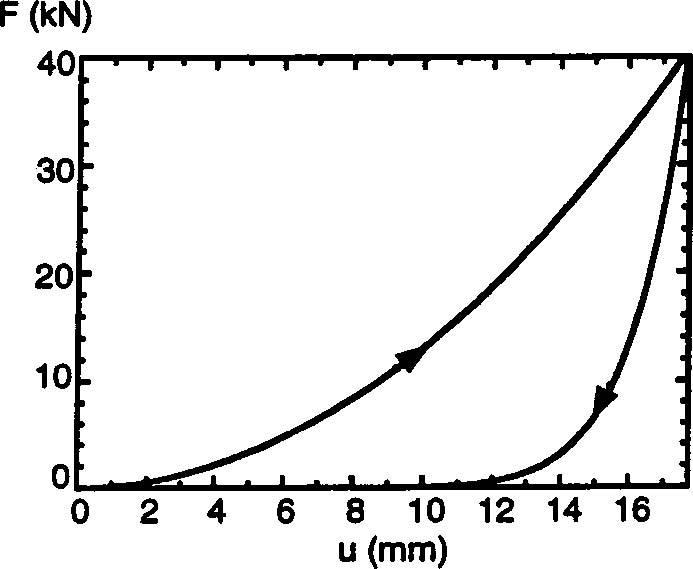
\includegraphics[scale=0.8]{ballmodel}
\caption{Schematic representation of a bat that is bent
and sheared.}\label{fig:ballmodel}
\end{figure}
\end{center}

The baseball-bat collision is violent and involves large forces
which act over a very short time and which compress the ball to a fraction of its normal size.

with an equal reactive force on the bat.
Such forces distort bat and ball: The ball is compressed to about  half of its original diameter,
the bat is compressed about $1/25$ as much\cite{K.Adair2002}.

The collision is highly inelastic, with $65\%$ of the energy is lost to friction,
found in the static measurements of Kirkpatrick designed to address the ball-bat collision\cite{Kirkpatrick1963}.

The phenomenological embodiment of this inelasticity is the coefficient of restitution,
which we denote by the symbol $e_0$.
It is defined as the ratio of relative speeds after to before
the collision of the ball with a perfectly rigid object:

\begin{equation}
\mathrm{coefficient\ of\  restitution}:e_0\equiv \frac{v_{rel,f}}{v_{rel,b}}
\end{equation}

With this definition, the fraction of the initial center of mass energy that is dissipated equals $1-e_0^2$.



The process of collision can be understood with the
help of the dynamic stress-strain hysteresis curve shown in
Fig.\ref{fig:ballmodel},
in which the path taken during the compression phase
is different from that taken during the expansion phase. The area bounded by the two curves is the energy dissipated

\begin{equation}
E_{lost}=\oint F(u)\dd u \label{equ:elost}
\end{equation}

Defining $u$ as the compression of the radius of the ball, we parametrize the hysterisis curve as compression:
\begin{eqnarray}
\left\{
\begin{array}{ll}
compression:&F(u)=k_1 u^\alpha \\
expansion:&F(u)=k_2 u^\beta
\end{array}\right.\label{equ:dynamicofcollision}
\end{eqnarray}

where generally $\beta \geq \alpha$.
Since the fractional energy loss is $1-e_0^2$,
 Eqs.\ref{equ:elost} and \ref{equ:dynamicofcollision}
 lead to

\begin{equation}
\beta=\frac{1+\alpha}{e_0^2}-1
\end{equation}

The parameter $k_2$ is determined from the remaining parameters by equating the two expressions for the force at the point of maximum compression. Our model therefore has three parameters: the compression constant $k_1$, the compression exponent $a$ and $e_0$.
The parameter $k_1$ essentially sets the overall time scale for the collision, whereas a determines
the variation of the collision time with initial impact speed. For a linear spring ($\alpha=1$) with no losses, the collision
time is half of the oscillation period of the spring independent of the impact speed, whereas for $a>1$ the collision
time decreases with increasing impact speed.

\subsection{Model of Collision}

We are now in a position to formulate the collision problem.

We assume that the ball impacts the bat on the $k$th slice.
The formalism could easily be generalized to allow for a force spread over several slices. The force that the ball and bat mutually exert on each other depends on
the compression of the radius of the ball according to
Eq.\ref{equ:dynamicofcollision}.
We take $u$ to be the separation between the surface of the bat $y_k(t)$ and the center of the ball $y_{ball}(t)$ but offset by the natural radius $R_{ball}$ so that $u=0$ corresponds to no compression.
As discussed in the preceding section, the functional
form of that force depends on whether the spring is compressing
($\dot{u}<0$) or expanding ($\dot{u}>0$). Putting all this together,
the complete dynamics of the collision are contained
in the equations

\begin{eqnarray}
y_i{t}=\sum_n a_n(t) y_{ni}\\
\ddot{a}_m(t)+\omega^2_m a_m(t)=\frac{1}{\rho \bar{A}}\sum_iF_i(t)y_{mi}\\ \label{equ:addot}
m_{ball}\ddot{y}_{ball}=-F(u(t))\\
u(t)=R_{ball}-(y_{ball}(t)-y_k(t))
\end{eqnarray}

Together with the normal modes, the force law, and the initial conditions. For the latter, we take $t=0$ to be the time when
the ball and bat come into contact for the first time
$u=0, \ \dot{u}<0$, at which time the ball and the rigid-body modes of the bat each have initial velocities which must be specified. Under typical conditions, the ball and bat (at the impact point) are initially moving in opposite directions. Since the bat is assumed not to be vibrating prior to the collision, we
set $a_n(0)=\dot{a}_n(0)=0$ for the true vibrational modes. Standard fourth-order Runge-Kutta is used to integrate the
coupled differential equations numerically, using a time grid adjusted to give stable results. For a typical
collision lasting less than 1 ms, a mesh of $5 \mu s$ is more than adequate. When the ball and bat separate ($u=0,\dot{u}=0$)
the force goes to zero,the bat vibrates freely, and the ball exits with constant velocity $v_f$ .

\subsection{Calculation by Energy Conservation}

The total energy conserves in the whole process of collision between the ball and the bat. That is, once the ball and
bat separate, the initial kinetic energy of the ball-plus-bat system is shared among the final kinetic energy of the ball, the energy contained in rigid-body modes (translation and rotation)of
the bat, vibrational energy of the bat, and energy
lost in the compression and expansion of the ball. It is useful to develop some formulas for the partitioning of the energy of the bat among the normal modes.Theenergy contained in the $n$th vibrational mode is given by

\begin{equation}
E_n=\frac{1}{2}\rho \bar{A}(\dot{a}_n^2{\tau}+\omega^2_n a^2_n(\tau))
\end{equation}

where t is the collision time. We define the force profile
$\mathcal{F}\equiv F/\mathcal{I}$, where $\mathcal{I}$ is the total impulse imparted to the ball in
the collision, so that

$$\int^\tau_0 \mathcal{F}(t)\dd t=1$$

Assuming
$a_n(0)=\dot{a}_n(0)=0$,
the solution to Eq.\ref{equ:addot} can be written

$$a_n(\tau)=\frac{y_{nk}\mathcal{I}}{\rho \bar{A} \omega_n}\int^\tau_0\mathcal{F}(t)\sin \omega_n(\tau-t)\dd t$$
from which we derive

\begin{eqnarray}
E_n&=&\frac{\mathcal{I}^2}{2m_{ball}}R_n \nonumber \\
R_n&=&[\frac{y^2_{nk}m_{ball}}{\rho \bar{A}}]g(\omega_n) \\
g(\omega_n)&\equiv&|\int^\tau_0\mathcal(t)e_{i\omega_n t\dd t}|^2
\end{eqnarray}

These equations define $R_n$, which is a dimensionless parameter that is proportional to the energy transferred to the $n$th normal mode as a result of the collision.

In general, one can interpret $R_n$ as the ratio of ball mass to an effective bat mass. It depends in part on the squared amplitude of the mode at the impact point ($y_{nk}^2$).

\subsection{The Exit Speed of the Ball}

Our goal is to calculate the exit speed of the ball $v_f$.
We will find it useful to develop
some formulas relating $v_f$ to the initial speed of the
ball $v_{ball}$ and the initial speed of the bat at the impact point $v_{bat}$.
We do this first for a rigid bat. We proceed by eliminating all but the two
zero-frequency rigid-body modes, which correspond to the
recoil of the center of mass of the bat and the rigid rotation
of the bat about its center of mass. The calculation of $R$ for
these modes is straightforward, resulting in

%公式15
\begin{equation}
R_0=\frac{m_{ball}}{M}[1+(\frac{z_k-z_{CM}}{r_\gamma})^2]
\end{equation}

where $z_k$ is the location of the $k$th slice (the impact point)
and $r_\gamma$ is the radius of gyration
($I_{CM}=Mr^2_\gamma$). We easily arrive
at rigid approximation:

%公式16

\begin{equation}
v_f=[\frac{e_0-R_0}{1+R_0}]v_{ball}+[\frac{e_0+1}{1+R_0}]v_{bat}
\end{equation}

This result is expected to be valid whenever the energy contained in vibrations is small, such as when the impact point is
close to one or more nodes of the lowest-frequency modes. This formula conserves momentum and angular momentum and energy.

We attempt to generalize this result for the case in which vibrations are included.
We start with the simple case in
which there are vibrations in the bat but no dissipation in the
ball(i.e., $e_0=1$).
Under such conditions, one can rigorously
show that the correct formula for the exit speed of the ball is given by

%公式17
\begin{equation}
e=1: \ \ v_f=[\frac{1-\sum_n R_n}{1+\sum_nR_n}]v_{ball}+[\frac{2}{1+\sum_n R_n}]v_{bat}
\end{equation}

Where the sum is over all the normal modes
(rigid and vibrational),
The most general case can be cast in the form
general case:
\begin{equation}
\mathrm{general\ case}: v_f=[\frac{e_{eff}-R_0}{1+R_0}]v_{ball}+
[\frac{e_{eff}+1}{1+R_0}]v_{bat}\label{equ:general}
\end{equation}

whereas $e_0$ is the coefficient of restitution for the collision of the ball with a rigid surface and therefore it's a
property of the ball alone, $e_{eff}$ is an effective coefficient of restitution for
the collision of the ball with a flexible bat. The effective coefficient of restitution has the desired
properties that it reduces to $e_0$ in the limit that vibrations are neglected and it satisfies the definition of coefficient of restitution.

\subsection{Comparison of Normal and Corked Bat}

\begin{center}
\begin{figure}[htpb]
\centering
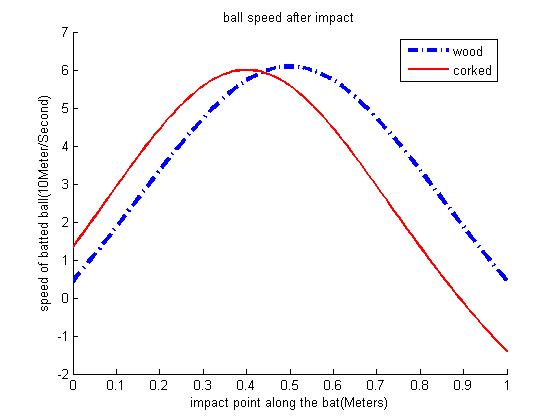
\includegraphics[scale=0.5]{corked}
\caption{$v_f$ varies by location of impact point of normal and corked bat}\label{fig:corked}
\end{figure}
\end{center}

A graph of Eq.\ref{equ:general} was drawed with data measured by H.Brody\cite{H.Brody1990} listed in Table.\ref{tab:corked}.
The curve of the equation are showed in Fig.\ref{fig:corked}.
The effective COR are setted to equal value, for there are few changes in effective COR ($e_{eff}$)  caused by corked bat
according to Alan Nathan' experiment\cite{NathanDecember12004}.

\begin{centering}
\begin{table}
\centering
\caption{Properties of bat}\label{tab:corked}
\begin{tabular}{lll}
 \hline
        &normal bat & corked bat\\
 \hline
 mass&0.846 kg & 0.800 kg\\
 length&0.84 m & 0.84 m\\
 distance of CM from handle &0.51 m & 0.40 m\\
 moment of inertia about CM&0.047 $kg\cdot m^2$ & 0.040 $kg\cdot m^2$\\
 effective COR $e_{eff}$&0.40 & 0.40\\
 \hline
\end{tabular}
\end{table}
\end{centering}


It is obvious from Fig.\ref{corked} that the maximum $v_f$ of corked bat is slightly less thant that of a normal bat, which improves that corking bat does not enhances the ``sweet spot'' effect in terms of velocity increasement.

\subsection{Physical Explanation}

The main influence in $v_f$ caused by corking a bat is the value of mass
and location of center of mass,
suppose that we always hit the ball at sweet point.
The bat shakes slightly when hitting at the sweet point,
and there's little energy disspation in vibration energy of the bat.

The corked bat has a better flexibility,
but integrity of the bat is lost.

\subsection{Reason for Prohibition of Corking}
Since corking doesn't enhance "sweet spot" effect,then how does unfairness come?
\begin{enumerate}
\item Reaction time of the batter is prolonged for the velocity of the bat can be larger. Since
moment of inertia of the bat with respect to the handle point is reduced by corking, the
bat can be swung faster with the same force. So the batter will have more time for reaction and control of the bat, thus the batter can have a better performance with the same skill.
\item The bat is easier for the batter to control since the mass is reduced.
\end{enumerate}

So the corked bat has a beneficial effect for a contact-type hitter, who is
just trying to meet the ball squarely rather than get the highest batted ball speed.

\subsection{Conclusion}
Corking a bat does not enhance ``sweet spot''effect, according to the result of the augmented model in which vibration is taken into account.Two main reasons for Major League to prohibit corking is that the reaction time of the batters are prolonged and that corked bats are easier to control,which help the batter make a good performance.

%===========================\input{WoodvsAluminumBat}===============================
\section{Wood vs Aluminum Bat}
In this part,we will work out the different behavior for wood (ash) and metal (aluminum) bat on the basis of the augmented
model.
\subsection{Differences in Parameters}

The main differences between wood and aluminum bat are mass, location of center of mass, moment of inertia with respect to
center of mass, and the effective coefficient of restitution $e_{eff}$.

Effective COR $e_{eff}$ is an important factor which
actually stand for the elasticity of the bat. The elasticity of a bat is described by Young's modulus and shear modulus,
so in fact $e_{eff}$ is a combination of the two modulus.Thus,we are able to take into account the difference in vibration
of the bat,which is mainly determined by Young's modulus and shear modulus.
%Definition补充定义有效恢复系数Effective coefficient of restitution $e_eff$ is an effective coefficient of restitution for the collision of the ball with a flexible bat rather than a stationary wall,which is the definition of COR.

Parameters of the wood and aluminum bat:
\begin{center}
\begin{table}
	\caption{Properties of bat}\label{tab:thi}
\begin{tabular}{lll}
\hline
    & wood bat &aluminum bat\\
\hline
mass&0.846 kg&0.825 kg\\
length&0.84 m& 0.81 m\\
distance of CM from handle&0.51 m& 0.46 m\\
moment of inertia about CM&0.047 $kg\cdot m^2$& 0.046 $kg\cdot m^2$\\
effective COR $e_{eff}$&0.40& 0.58\\
\hline
\end{tabular}
\end{table}
\end{center}

We take the initial velocity of the ball and the bat as:$v_{ball}=8 m/s$,$v_{bat}=4 m/s$.

\subsection{Calculation and Analysis}
Substitute these values for parameters in the equation we get above,the final velocity of ball $v_f$ tuned a explicit
function of the distance of impact point to the handle $z_k$.We draw a graph of this function for both kinds of bats,
see figure . %图号
%插图:figure :$v_f$ varies by $z_k$.

\begin{center}
\begin{figure}[htpb]
\centering
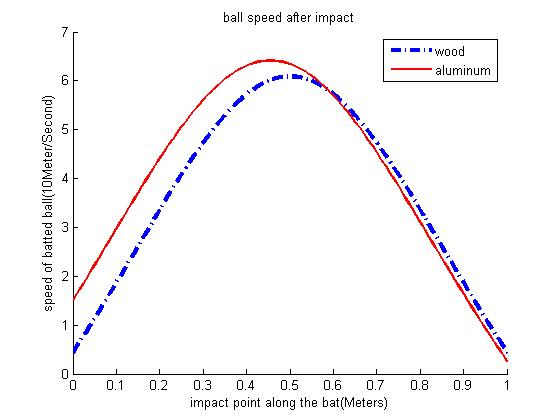
\includegraphics[scale=0.4]{aluminium}
\caption{$v_f$ varies by $z_k$}\label{fig:aluminium}
\end{figure}
\end{center}

From the graph,we note that peak value of $v_f$ of aluminum bat is a bit higher than that of wood bat,and in a large zone
near the handle the $v_f$ of aluminum bat is also a higher than that of wood bat.At the peak point (sweet spot),the
aluminum outperforms wood by about $5\%$,in term of velocity.

\subsection{Conclusion}
Notable differences between aluminum bat and wood bat are seen in the prediction of the augmented model.Overall,the
aluminum bat outperforms wood bat,and at the sweet  spot,the aluminum outperforms wood by about $5\%$.You may say the
difference is small,but it is never negligible in an regulation game,the foremost principle of which is justice.
This enhanced "sweet spot" effect of metal bat is the main reason for its prohibition by Major League Baseball.

In addition,since the moment of inertia of and mass of aluminum bat is smaller,reaction time will be prolonged and it
becomes easier for batter to control the bat,making the injustice even more serious.

%====================================\input{StrengthsandWeaknesses}============================================
\section{Strengths and Weaknesses}

\subsection{Strengths}
\begin{enumerate}
\item Vibration of bat is taken into account so that the accuracy of the model can be fairly good.
\item Physical explanation is put forward besides the model for a better understanding of the collision process.
\item Figures are used for explanation of the problem,thus making it more intuitive and easier to understand.
\end{enumerate}

\subsection{Weaknesses}
\begin{enumerate}
\item The ball is actually nonlinear when deformation of the ball go beyond a certain limit.The approximation of linear model turned to be flawed when the force applied on the ball become very large.
\item Effective coefficient of restitution can not be calculated accurately.This affect the accuracy of the result of the model.
\end{enumerate}

%========================Bibtex
\newpage
\bibliography{baseballref}%放在|begin{document}前不可用
\bibliographystyle{ieeetr}%引用格式 ieeetr
%\fi
%\end{CJK}

\end{document}
